\documentclass[border=10pt]{standalone}

\usepackage{tikz}
\usepackage{tikzsymbols}
\usetikzlibrary{calc,patterns,shapes.geometric}

\def\centerarc[#1](#2)(#3:#4:#5){\draw[#1] ($(#2)+({#5*cos(#3)},{#5*sin(#3)})$) arc (#3:#4:#5);}

\begin{document}
	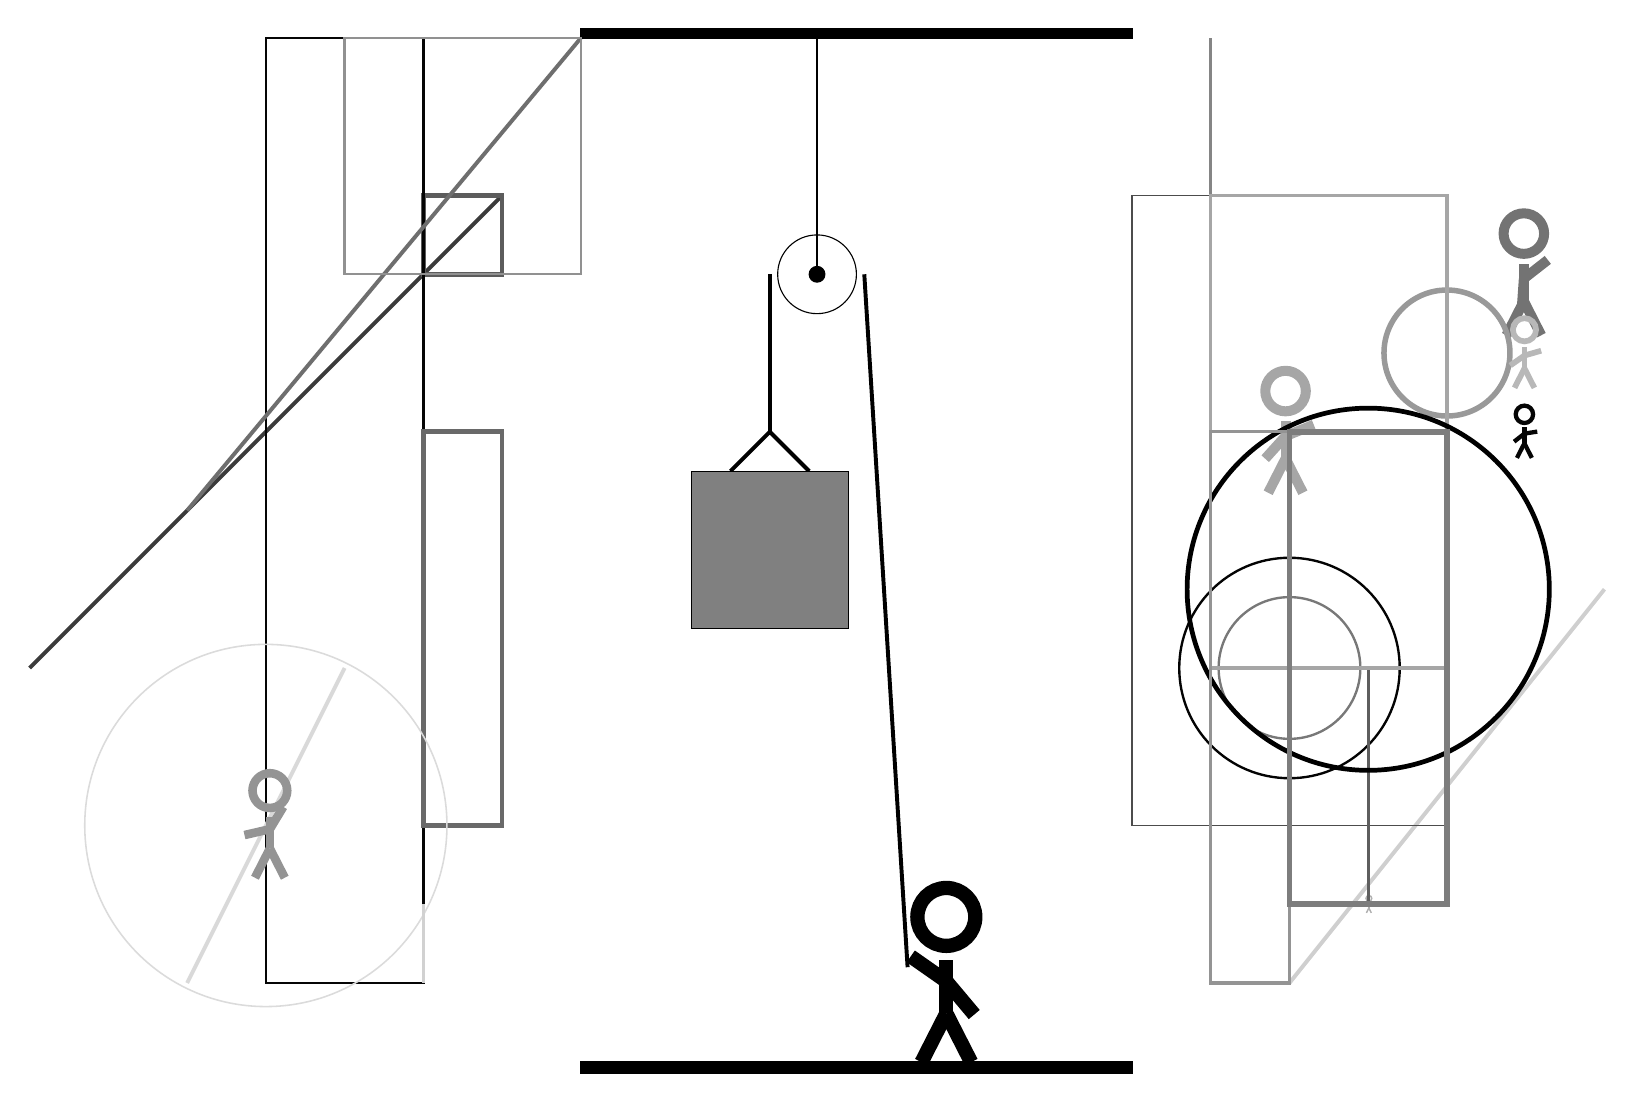
\begin{tikzpicture}
		%%%%% START %%%%%
		
		\draw[fill=black] (-2, 10) rectangle (5, 10.125);
		
		\draw (1, 7) circle (0.5);
		\draw[fill=black] (1, 7) circle (0.1);
		\draw (1, 10) -- (1, 7);
		
		\draw[line width=0.5mm] (-0.1, 4.5) -- (0.4, 5.0) -- (0.9, 4.5);
		\draw[fill=black!50] (-0.6, 4.5) rectangle (1.4, 2.5);
		
		\draw[line width=0.5mm] (0.4, 7) -- (0.4, 5.0);
		\centerarc[line width=0.5mm](1, 7)(0:180:0.6);
		\draw[line width=0.5mm](1.6, 7) -- (2.15, -1.8);
		
		\draw[line width=0.5mm, color=black!77](-3, 8) -- (-9, 2);
		
		\draw [line width=0.3mm, color=black!99](7, 2) circle (1.4);
		\node[line width=0.2mm, color=black!31] at (8, -1) {\Strichmaxerl[1][15][53]};
		\draw [line width=0.3mm, color=black!53](7, 2) circle (0.9);
		\draw[line width=0.5mm, color=black!19](7, -2) -- (11, 3);
		
		\draw[line width=0.6mm, color=black!64] (-3, 7) rectangle (-4, 8);
		\draw[line width=0.3mm, color=black!98] (-4, 10) rectangle (-6, -2);
		\node[line width=0.2mm, color=black!55] at (10, 7) {\Strichmaxerl[7][86][38]};
		\draw[line width=0.5mm, color=black!57](-2, 10) -- (-7, 4);
		\draw [line width=0.7mm, color=black!40](9, 6) circle (0.8);
		\draw[line width=0.5mm, color=black!15](-5, 2) -- (-7, -2);
		\node[line width=0.6mm, color=black!98] at (10, 5) {\Strichmaxerl[3][38][9]};
		\draw[line width=0.6mm, color=black!59] (-4, 5) rectangle (-3, 0);
		
		\draw[line width=0.4mm, color=black!70] (6, 2) rectangle (8, 2);
		\draw[line width=0.4mm, color=black!48] (6, 10) rectangle (6, 8);
		\draw[line width=0.2mm, color=black!70] (5, 0) rectangle (9, 8);
		\draw[line width=0.3mm, color=black!43] (-2, 7) rectangle (-5, 10);
		\node[line width=0.6mm, color=black!28] at (10, 6) {\Strichmaxerl[4][35][16]};
		\draw[line width=0.4mm, color=black!63] (7, -1) rectangle (8, 2);
		
		\draw [line width=0.2mm, color=black!14](-6, 0) circle (2.3);
		\draw[line width=0.4mm, color=black!35] (6, 8) rectangle (9, 2);
		
		\draw[line width=0.3mm, color=black!18] (-4, -2) rectangle (-4, -1);
		\node[line width=0.2mm, color=black!35] at (7, 5) {\Strichmaxerl[7][48][22]};
		\draw [line width=0.6mm, color=black!100](8, 3) circle (2.3);
		\draw[line width=0.4mm, color=black!42] (6, -2) rectangle (7, 5);
		
		\node[line width=0.3mm, color=black!42] at (-6, 0) {\Strichmaxerl[6][13][59]};
		\draw[line width=0.7mm, color=black!51] (7, -1) rectangle (9, 5);
		
		\node at (2.6, -1.9) {\Strichmaxerl[10][-35][-50]};
		
		\draw[fill=black] (-2, -3) rectangle (5, -3.15);
		
		%%%%% END %%%%%
	\end{tikzpicture}
\end{document}